% -----------------------------------------------
% Template for ISMIR 2014
% (based on earlier ISMIR templates)
% -----------------------------------------------

\documentclass{article}
\usepackage{ismir2014,amsmath,cite}
\usepackage{graphicx}
% \usepackage{hyperref}
\usepackage{booktabs}
\usepackage{brian}

% Title.
% ------
\title{Analyzing song structure with spectral clustering}

% Single address
% To use with only one author or several with the same address
% ---------------
%\oneauthor
% {Names should be omitted for double-blind reviewing}
% {Affiliations should be omitted for double-blind reviewing}

% Two addresses
% --------------
%\twoauthors
%  {First author} {School \\ Department}
%  {Second author} {Company \\ Address}

% Three addresses
% --------------
\threeauthors
  {First author} {Affiliation1 \\ {\tt author1@ismir.edu}}
  {Second author} {\bf Retain these fake authors in\\\bf submission to preserve the formatting}
  {Third author} {Affiliation3 \\ {\tt author3@ismir.edu}}

% Four addresses
% --------------
%\fourauthors
%  {First author} {Affiliation1 \\ {\tt author1@ismir.edu}}
%  {Second author}{Affiliation2 \\ {\tt author2@ismir.edu}}
%  {Third author} {Affiliation3 \\ {\tt author3@ismir.edu}}
%  {Fourth author} {Affiliation4 \\ {\tt author4@ismir.edu}}

\begin{document}
%
\maketitle
%
\begin{abstract}
Many approaches to analyzing the structure of a musical recording involve detecting
sequential patterns within a self-similarity matrix derived from time-series features.
Such patterns ideally capture repeated sequences, which then form the building blocks
of large-scale structure.

In this work, techniques from spectral graph theory are applied to analyze repeated
patterns in musical recordings.  The proposed method produces a low-dimensional
encoding of repetition structure, and exposes the hierarchical relationships among
structural components at differing levels of granularity.  Finally, we demonstrate how
to apply the proposed method to the task of music segmentation.
\end{abstract}
%
\section{Introduction}\label{sec:introduction}
Detecting repeated forms in audio is fundamental to the analysis of structure in many 
forms of music.  While small-scale repetitions --- such as each instance of an
individual chord --- are simple to detect, accurately combining multiple 
small-scale repetitions into larger structures is a challenging algorithmic task.
Much of the current research on this topic begins by calculating local, frame-wise
similarities over acoustic features (usually harmonic), and then searching for
patterns in the all-pairs self-similarity matrix~\cite{foote2000automatic}.

In the majority of existing work on structural segmentation, the analysis is
\emph{linear}, in the sense that the representation does not explicitly encode nesting
or hierarchical structure in the repeated forms.  Instead, novelty curves are commonly
used to detect when one section transitions into the
next~\cite{serra2012unsupervised}. 

% TODO:   2014-05-06 08:09:31 by Brian McFee <brm2132@columbia.edu>
%  why are we doing this work?
%   one level of segmentation is never enough
%   we want a full parse of the recording
%   how do nested structures relate to each-other?


\subsection{Our contributions}
In this paper, we formulate the structure analysis problem in the context of spectral
graph theory.  By combining local sequence information with long-term repeated forms,
and analyzing the eigenvectors of the resulting graph Laplacian, we produce a compact
representation that effectively encodes repetition structure at multiple levels of
granularity.  To effectively link repeating sequences, we formulate an optimally
weighted combination of local timbre consistency and long-term repetition descriptors.

To motivate the analysis technique, we demonstrate its use for the
standard task of flat structural annotation.  However, we emphasize that the approach
itself could have more general applications in analyzing hierarchical structure.

\subsection{Related work}

The structural repetition features used in this work are inspired by those of
Serr\`{a}~\etal~\cite{serra2012unsupervised}, wherein structure is detected by 
applying filtering operators to a lag-skewed self-similarity matrix.  The primary
deviation in this work is the graphical interpretation and subsequent analysis of 
the filtered self-similarity matrix.

% kaiser proposed a method to combine input features for novelty detection
% our method is different: we optimally combine local timbre information with global
% harmonic repetition
Recently, Kaiser~\etal demonstrated a method to combine tonal and timbral features for
structural boundary detection~\cite{kaiser2013simple}.  Whereas their method forms a
novelty curve from the combination of multiple features, our feature combination
operates slightly differently, and uses local timbre consistency to connect sequences
of long-range tonal repetitions.

% grohganz used spectral analysis of self-similarity to detect diagonals
% but our approach is more direct, analyzes the diffusion process rather than the
% graph itself
Our general approach is similar in spirit to that of Grohganz 
\etal~\cite{grohganz2013converting}, in which diagonal bands 
of a self-similarity matrix are expanded into block structures by 
spectral analysis.  Their method analyzed the spectral decomposition of the 
self-similarity matrix directly, whereas the method proposed here operates on the
graph Laplacian.  Similarly, Kaiser and Sikora applied non-negative matrix
factorization directly to a self-similarity matrix in order to detect blocks of
repeating elements~\cite{kaiser2010music}.  
As we will demonstrate, the Laplacian provides a more direct means to
expose block structure at multiple levels of detail.

\section{Encoding repeated structure}
% Begin with nearest-neighbor linkage in some feature space
% Apply diagonal majority vote filtering
% Add the conveyor belt links
% Compute the graph laplacian, observe magic

Let $X = [x_1, x_2, \dots, x_n] \in \R^{d\times n}$ denote a $d$-dimensional time
series feature matrix, \eg, a chromagram or sequence of Mel-frequency cepstral 
coefficients.  As a first step toward detecting and representing repetition structure, 
we form a \emph{binary recurrence matrix} $R \in \{0,1\}^{n\times n}$, where 
\begin{equation}
R_{ij}(X) \defeq \begin{cases}
1 & x_i, x_j \text{ are mutual $k$-nearest neighbors}\\
0 & \text{otherwise},
\end{cases}
\end{equation}
and $k$ is a linkage parameter controlling the degree of connectivity in $R$.

% FIXME: cite for recurrence matrix

If $X$ sufficiently captures the qualities of interest, and $k$ is large
enough, then repeated structures should appear as diagonal stripes in $R$.
In practice, it is beneficial to apply a smoothing filter to $R$ to suppress erroneous
links, and fill in gaps.  Here, we apply a windowed majority vote to each diagonal of
$R$, resulting in the filtered matrix $R'$:
\begin{equation}
R'_{ij} \defeq \maj\left\{ R_{i+t, j+t} \given t \in -w, -w+1, \dots, w\right\},
\label{filtered-rep}
\end{equation}
where $w$ is a discrete parameter that defines the minimum length of a valid
repetition sequence.

\subsection{Internal connectivity}
The filtered recurrence matrix $R'$ can be interpreted as an unweighted, undirected 
graph, whose vertices correspond to samples (columns of $X$), and edges correspond 
to equivalent position within a repeated sequence. Note, however, that successive 
positions $(i, i+1)$ will not in general be connected in $R'$, so the constituent 
samples of a particular sequence will not be directly linked.

In order to facilitate the discovery of repeated sections, we modify $R'$ by 
adding links between adjacent samples $(i, i+1)$ and $(i, i-1)$, resulting in the
\emph{sequence-augmented graph} $R^+$:
\begin{eqnarray}
\Delta_{ij} &\defeq \begin{cases}
1 & |i - j| = 1\\
0 & \text{otherwise}
\end{cases},\\
R^+_{ij} &\defeq \max(\Delta_{ij}, R'_{ij})\label{pathmatrix}.
\end{eqnarray}
With appropriate normalization, $R^+$ can be interpreted as a Markov process
over samples, where at each step $i$, the process either moves to an adjacent
sample $i\pm1$, or a random repetition of $i$; a process exemplified by the 
Infinite Jukebox~\cite{infinitejukebox}.

\Cref{pathmatrix} explicitly combines local temporal connectivity with long-term
recurrence information.  Ideally, we would add connections only to pairs $\{i,j\}$
belonging to the same component, but of course, this information is hidden.  Rather,
by adding links along the first diagonals, the graph becomes fully connected.  
However, repeated sections will contain internal connectivity structure.  Let $i$ and
$j$ denote two repetitions of the same sample at different times; then $R^+$ should
ideally contain edges $\{i, i+1\}$, $\{i, j\}$, $\{i+1, j+1\}$, $\{j, j+1\}$.
Connections between unrelated blocks are likely to remain sparse, owing primarily to
cross-section links along the first diagonals.  

% $R^+$ encodes the coarse similarity structure
% For the purposes of musical structure analysis, we would like to produce a block
% matrix $C$, where $C_{i,j}$ indicates that $i$ and $j$ belong to the same structural
% component (\eg, $i$ and $j$ are both of type \emph{verse}).

\subsection{Balancing local and global linkage}
While the construction of \cref{pathmatrix} describes the intuition behind combining
local sequential connections with global repetition structure, it does not explicitly
model the balance between the two competing goals.  In particular, for long tracks
with many repetitions, the local connectivity structure may be washed out by
recurrence links, thereby obscuring the sequence structure we hope to reveal.

However, if we allow weights on the edges, then the combination can be parameterized 
by a weighting parameter $\mu \in [0, 1]$:
\begin{equation}
R^\mu \defeq \mu R' + (1 - \mu) \Delta. \label{weightedsum}
\end{equation}

This raises the question: how should $\mu$ be set?  Returning to the motivating
example of the random walk process, we opt for a process that on average, tends to
move in sequence or across (all) repetitions with equal probability.  In terms of
$\mu$, this indicates that we should optimize the combination such that the local
links achieve equivalent weight to the repetition links.  More precisely, for any 
frame $i$,
$$
\mu \sum_j R'_{ij} \approx (1-\mu) \sum_j \Delta_{ij} 
$$
Minimizing the average squared error between the two terms above leads to the
following quadratic optimization:
\begin{equation}
\min_{\mu \in [0, 1]} \frac{1}{2} \sum_i {(\mu d_i(R') - (1 - \mu)d_i(\Delta))}^2,\label{optweight}
\end{equation}
where $d_i(A) \defeq \sum_j A_{ij}$ indicates the degree (sum of incident edge-weights) 
of $i$ in $A$. By treating $d(\cdot) \defeq {[d_i(\cdot)]}_{i=1}^n$ a vector in 
$\R^n_+$, we obtain the solution to \cref{optweight} in closed form as
\begin{equation}
\mu^* = \frac{\langle d(\Delta), d(R') + d(\Delta)\rangle}{\|d(R') +
d(\Delta)\|^2}.\label{optweight:solution}
\end{equation}
Note that because $\Delta$ is fully connected, we always have $\|d(\Delta)\|^2 > 0$,
so $\mu^* > 0$.  Consequently, $R^\mu$ retains the full connectivity structure
of $R^+$, and remains connected even when $R'$ is empty.

\subsection{Edge weighting and feature fusion}
In the construction above, we rely upon a single feature representation $X$ to 
determine the self-similarity structure, and use constant edge weights for the
repetition and local edges.  The construction can generalize to support
feature-weighted edges by replacing $R'$ with a masked similarity matrix:
\begin{equation}
R'_{ij} \mapsto R'_{ij} S_{ij},
\end{equation}
where $S_{ij}$ denotes a non-negative affinity between frames $i$ and $j$, \eg,
a Gaussian kernel over feature vectors $x_i, x_j$.

Similarly, $\Delta$ can be replaced with a weighted variant.  However, in doing so,
care must be taken when selecting the affinity function.  In particular, the same
features used to detect repetition (typically harmonic in nature) may not work well
for local comparisons, since we may not expect successive frames to retain
harmonic similarity.  

Recent work has demonstrated that local timbre differences 
can provide an effective cue for structural boundary
detection~\cite{kaiser2013simple}.  This motivates the use of two contrasting feature
descriptors: harmonic features for detecting long-range repeating forms, and timbral
features for detecting local consistency.  We assume that these features are
respectively supplied in the form of affinity matrices $S^\text{rep}$ and
$S^\text{loc}$.  Combining these affinities with the detected repetition structure and
optimal weighting, we arrive at the \emph{sequence-augmented affinity matrix} $A$:
\begin{equation}
A_{ij} \defeq \mu R'_{ij} S^\text{rep}_{ij} + (1-\mu) \Delta_{ij} S^\text{loc}_{ij},\label{saam}
\end{equation}
where $R'$ is understood to be
constructed solely from the repetition affinities $S^\text{rep}$, and $\mu$ is
optimized by \eqref{optweight:solution} on the weighted affinity matrices.


\section{Algorithms}

The Laplacian is a fundamental tool in the field of spectral graph
theory, as can be interpreted as a discrete analog of a diffusion operator over the
vertices of the graph, and its spectrum can be used to characterize 
vertex connectivity~\cite{chung1997spectral}.  In this section, we describe in detail
how spectral clustering can be used to analyze the repetition graph constructed in the
previous section.

\subsection{Background: spectral clustering}
Let $D$ denote the diagonal \emph{degree matrix} of $A$: $D \defeq \diag(d(A))$.  
The \emph{symmetric normalized Laplacian} $L$ is defined as:
\begin{equation}
L \defeq I - D^{-1/2} A D^{-1/2}.\label{symlaplacian}
\end{equation}

The Laplacian forms the basis of spectral clustering, in which vertices are
represented in terms of the eigenvectors of $L$~\cite{von2007tutorial}.  More
specifically, to cluster a dataset into $m$ clusters, each point $t$ is represented as
the (normalized) vector of the $t$th coordinates of the first $m$ eigenvectors of $L$,
corresponding to the $m$ smallest eigenvalues.
The motivation for its use stems from the observation that the multiplicity of the bottom
eigenvalue $\lambda_0 = 0$ corresponds to the number of connected components in a
graph, and the corresponding eigenvectors $y_i \in \R^n$ encode membership of vertices
in components.

In the non-ideal case --- as we have with $A$ --- the graph is fully connected, so
$\lambda_0$ has multiplicity 1, and the bottom eigenvector $y_0$ trivially encodes 
membership in the graph. 
However, in the case of $A$, we expect there to be many components
with high intra-connectivity and relatively small inter-connectivity, \eg, at the
transition point between sections.  Spectral clustering is well-suited to detecting
and pruning these weak links, and it can be viewed as an approximation method for solving
normalized graph cut problems~\cite{von2007tutorial}.

\Cref{recurrence} illustrates an example of the encoding produced by spectral
decomposition of $L$.  Although the first eigenvector (column) is uninformative, 
the remaining bases clearly encode membership in the diagonal regions depicted in the 
affinity matrix.  
The resulting pair-wise frame similarities for this example is shown in \Cref{lowrank}, 
which clearly demonstrates the ability of this representation to iteratively reveal 
nested repeating structure.

\begin{figure*}[t]
\centering
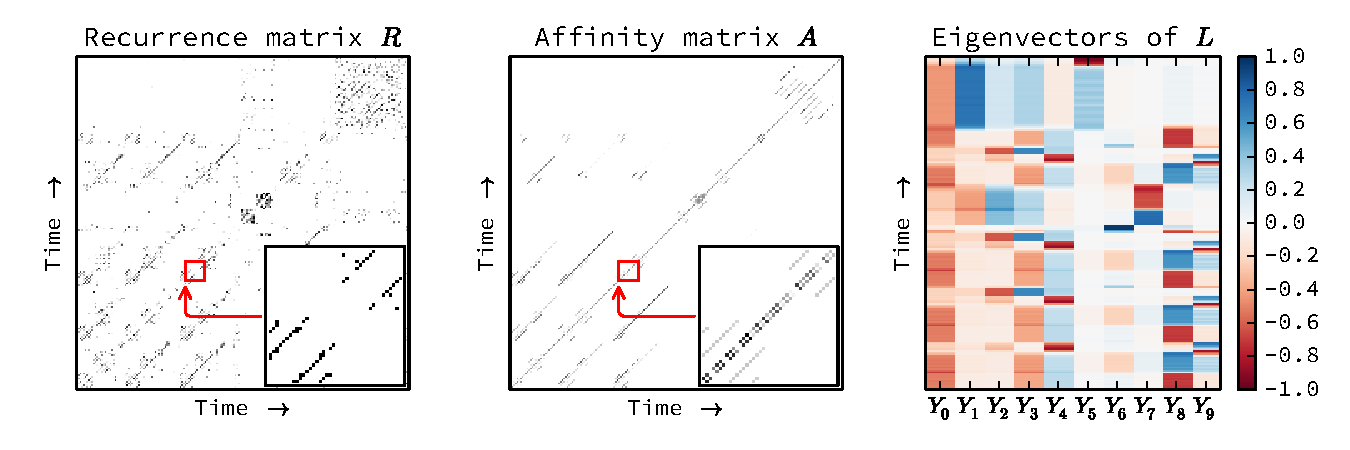
\includegraphics[width=\textwidth]{figs/recurrence}
\caption{Left: the recurrence matrix $R$ for \emph{The Beatles -- Come
Together}. Center: the sequence-augmented affinity matrix $A$.
Right: the first 10 basis features (columns), ordered left-to-right.  
The leading columns encode the primary structural components, while subsequent
components represent structural refinements.\label{recurrence}}
\end{figure*}

 
\begin{figure*}[t]
\centering
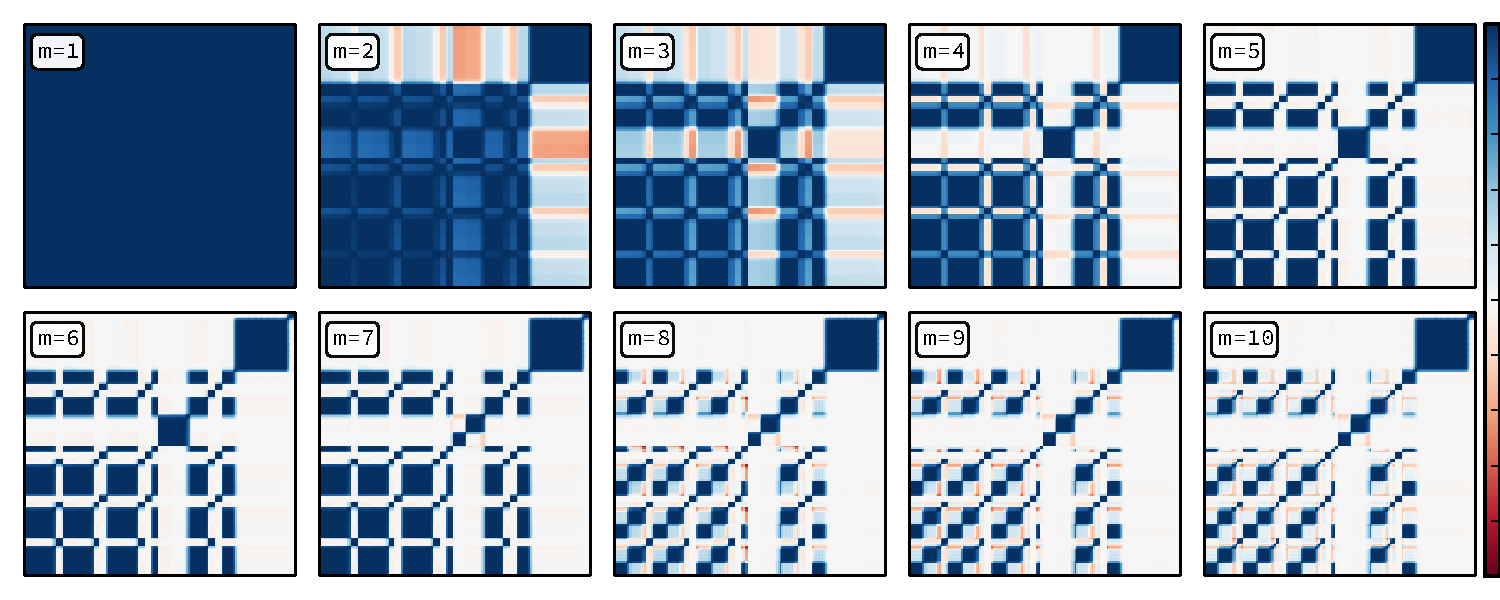
\includegraphics[width=\textwidth]{figs/lowrank}
\caption{Pair-wise frame similarity using the first $10$ components for \emph{The Beatles -- Come Together}.  The first
(trivial) component ($m=1$) captures the entire song, and the second ($m=2$) separates
the outro from the rest of the song.  Subsequent refinements separate the solo,
refrain, verse, and outro, and then refine each component into individual measures.\label{lowrank}}
\end{figure*}

To apply spectral clustering, we will apply $k$-means clustering to the (normalized) 
eigenvectors $Y \in \R^{n \times n}$ as features, where $M > 0$ is a 
specified maximum number of structural components.  By varying the number of
components $M$ --- equivalently, the dimension of the representation --- we can
directly adjust the resolution of the resulting segmentation.


\subsection{Boundary detection}
For a fixed number of segment types $m$, segment boundaries can estimated 
by clustering the columns of $Y$ after truncating to the first $m$ dimensions.
After clustering, segment boundaries are detected by searching for change-points in
the cluster assignments of $Y_{\cdot,t}$ and $Y_{\cdot,t+1}$.  This method is
formalized in \Cref{bd}.

\begin{algorithm}[t]
\caption{Boundary detection\label{bd}}
\begin{algorithmic}[1]
\REQUIRE{Repetition features $Y \in \R^{m \times n}$, }
\ENSURE{Boundaries $b$, frame-level segment labels $c$}\\

{\sc Boundary-Detect}$(Y)$
    \STATE{$\hat{y}_t \leftarrow Y_{\cdot, t} / \|Y_{\cdot, t}\|$}
    \COMMENT{Normalize columns $Y_{\cdot,t}$}
    \STATE{Run $k$-means on $\{\hat{y}_t\}_{i=1}^n$ with $k=m$}
    \STATE{Let $c_t$ be the cluster containing $\hat{y}_t$}
    \STATE{$b \leftarrow \{t \given c_t \neq c_{t+1}\}$} 
    \RETURN{$(b, c)$}
\end{algorithmic}
\end{algorithm}


\subsection{Laplacian structural decomposition}

To decompose an input song into its structural components, we propose a method, listed
as \Cref{lsd},
to find boundaries and structural annotations at multiple levels of structural
complexity.  This operates by first computing the Laplacian as described above, and
then iteratively increasing the set of eigenvectors for use in \Cref{bd}.  For $m=2$,
the first two eigenvectors --- corresponding to the two smallest eigenvalues of $L$
--- are taken.  In general, for $m$ types of repeating component, the bottom $m$
eigenvectors are used to label frames and detect boundaries.  The result is a sequence
of boundaries $B^m$ and frame labels $C^m$, for values $m \in 2, 3, \dots, M$.

Note that unlike most prior structural analysis algorithms, \Cref{lsd} does not produce a
single decomposition of the song, but rather a sequence of iteratively more complex 
decompositions.  This property can be valuable in visualization applications,
where a user may be interested in the relationship between structural components at
multiple levels.  Similarly, in interactive display applications, a user may wish to 
request more or less detailed analyses for a track.  Since complexity is controlled by
a single, discrete parameter $M$, this application is readily supported with a minimal
set of interface controls (\eg, a slider).

However, for standardized evaluation, the method must produce a single, flat
segmentation of the track.  Adaptively estimating the appropriate level of analysis in
this context is somewhat ill-posed, as different use-cases require different amounts of 
detail.  Here, we apply a simple selection criterion, based on the level of detail
commonly observed in standard datasets~\cite{harte2010towards,smith2011design}.  
First, we reduce the set of candidates to those in which the mean segment duration is 
at least some minimal threshold, in our case, 10 seconds.  
Subject to this constraint, we select the segmentation level $\tilde{m}$ whose 
frame-level annotations exhibit maximum entropy, thereby preferring solutions with 
approximately balanced distributions over the set of segment types.




\begin{algorithm}[t]
\caption{Laplacian structural decomposition\label{lsd}}
\begin{algorithmic}[1]
\REQUIRE{ Affinities: $S^\text{rep}, S^\text{loc} \in \R_+^{n\times n}$\\
maximum number of segment types: $M$}
\ENSURE{Boundaries $B^m$, frame labels $C^m$ for ${m \in 2\dots M}$}\\
{\sc LSD}$(S^\text{rep}, S^\text{loc})$
\STATE{$R' \leftarrow $ filtered recurrence matrix of $S^\text{rep}$ (\cref{filtered-rep})}
\STATE{$A \leftarrow $ sequence-augmented affinity matrix (\cref{saam})}
\STATE{$L \leftarrow I - D^{-1/2} A D^{-1/2}$}
\FOR{$m \in 2, 3, \dots, M$}
    \STATE{$Y \leftarrow$ bottom $m$ eigenvectors of $L$}
    \STATE{$(B^m, C^m) \leftarrow \text{\sc Boundary-Detect}(Y)$}
\ENDFOR{}
\RETURN{$\{(B^m, C^m)\}_{m=2}^M$}
\end{algorithmic}
\end{algorithm}

% For each m in 2 .. M:
% m <- argmax gap
% compute segment centroids over boundaries[m], and cluster by k-means with k=m
% return boundary times and segment labels

\section{Experiments}
To evaluate the proposed method quantitatively, we compare boundary detection and
structural annotation performance on two standard datasets.  We evaluate the
performance of the method using the automatic complexity estimation described above,
as well as performance achieved for each fixed value of $m$ across the dataset.

Finally, to evaluate the impact of the complexity estimation method, we compare to an
oracle model. For each track, a different $m^*$ is selected to maximize the
evaluation metric of interest.  This can be viewed as a simulation of interactive
visualization, in which the user has the freedom to dynamically adapt the level of
detail until she is satisfied.  Results in this setting may be interpreted as
measuring the best possible segmentation within the set of predictions made by
\Cref{lsd}.

\subsection{Data and evaluation}
Our data is comprised of two sources:
\begin{description}
\item[Beatles-TUT:\footnote{\texttt{http://www.cs.tut.fi/sgn/arg/paulus/structure.html}}]
174 structurally annotated tracks from the Beatles corpus.  In this set, a single
annotation is provided for each track, and annotations generally correspond to
functional components (\eg, \emph{verse}, \emph{refrain}, or \emph{solo}).
\item[SALAMI:] 735 tracks from the SALAMI corpus~\cite{smith2011design}.  This corpus
spans a wide range of genres and instrumentation, and provides multiple
annotation levels for each track.  We report results on \emph{functional},
% \emph{large-scale}, 
and \emph{small-scale} annotations.
\end{description}

In each evaluation, we report the $F$-measure of boundary detection at 0.5-second and
3-second windows.  To evaluate structural annotation accuracy, we report pairwise frame 
classification $F$-measure~\cite{levy2008structural}.  
For comparison purposes, we also report scores achieved by the method of 
Serr\`{a} \etal~\cite{serra2014unsupervised}.

\subsection{Implementation details}
All input signals are sampled at 22050Hz (mono), and analyzed with a 2048-sample FFT window
and 512-sample hop.  Repetition similarity matrices $S^\text{rep}$ were 
computed by first extracting log-power constant-Q spectrograms over 72 bins, ranging 
from $C2$ (32.7Hz) to $C8$ (2093.0Hz). Constant-Q spectrograms were generated by a 
down-sampling method similar to that of Sch{\"o}rkhuber and 
Klapuri~\cite{schorkhuber2010constant}.  

Constant-Q frames were mean-aggregated between detected beat events, and stacked using 
time-delay embedding with one step of history, as in~\cite{serra2014unsupervised}.
Similarity matrices were then computed by applying a Gaussian kernel
\[
S^\text{rep}_{ij} \defeq \exp\left(-\frac{1}{2\sigma^2}\|x_i - x_j\|^2\right)
\]
to each pair of beat-synchronous frames $i$ and $j$.
The bandwidth parameter $\sigma^2$ was estimated by computing the average 
squared distance between each $x_i$ and its $k$th nearest neighbor, with 
$k$ set to $1 + \lceil 2\log_2 n\rceil$.  The same $k$ was used to connect nearest
neighbors when building the recurrence matrix $R$, with the additional constraint that
frames cannot link to neighbors within 3 beats of each-other, which prevents
self-similar connections within the same measure. The majority vote window was set to
$w=17$.

Local timbre similarity $S^\text{loc}$ was computed by extracting the first 13 Mel
frequency cepstral coefficients (MFCC), mean-aggregating between detected beats, and
then applying a Gaussian kernel as done for $S^\text{rep}$.\footnote{All methods were implemented in Python, and source code will be made freely available upon publication.}

\subsection{Results}
The results of the evaluation are listed in
\Cref{results:beatles,results:salami:func,results:salami:small}.  For each fixed value
of $m$, the resulting scores are indicated as $L_m$.  $L$ indicates the automatic
maximum-entropy selector, and $L^*$ indicates the best possible $m$ for each metric
independently.

As a common trend across all data sets, the automatic $m$-selector often achieves results
comparable to the best fixed $m$.  However, it is consistently outperformed by the 
oracle model $L^*$, indicating that although the output of \Cref{lsd} often contains 
accurate solutions, the automatic selector does not always choose them.

In the case of SALAMI (small), the automatic selector performs dramatically worse than
many of the fixed-$m$ methods, which may be explained by the relatively different
statistics of segment durations and numbers of unique segment types in the small-scale
annotations as compared to Beatles and SALAMI (functional).

To investigate whether a single $m$ could simultaneously optimize multiple evaluation
metrics for a given track, we plot the confusion matrices for the oracle selections on
SALAMI (functional) in
\Cref{mconfusion}.  While there does appear to be a correlation, we observe that the
best $m$ to optimize $F_3$ is typically larger than those for $F_0.5$ (indicated by
the mass in the lower triangle of the left plot) or $F_\text{pair}$ (indicated by the
upper triangle of the right plot).  This corroborates previous observations that even
within the context of boundary detection, the 0.5-second and 3.0-second metrics
evaluate qualitatively different objectives~\cite{smith2013meta}.  Consequently, it may be
beneficial in practice to provide annotations at multiple resolutions, rather than a
single, fixed resolution.

\begin{table}
\centering
\caption{ Beatles (TUT)\label{results:beatles}}
\begin{tabular}{lrrr}
\toprule
Method & $F_{0.5}$ & $F_3$ & $F_\text{pair}$\\
\midrule
$L_2$   & 0.307 $\pm$ 0.14 & 0.429 $\pm$ 0.18   & 0.576 $\pm$ 0.14\\
$L_3$   & 0.303 $\pm$ 0.15 & 0.544 $\pm$ 0.17   & 0.611 $\pm$ 0.13\\
$L_4$   & 0.307 $\pm$ 0.15 & 0.568 $\pm$ 0.17   & 0.616 $\pm$ 0.13\\
$L_5$   & 0.276 $\pm$ 0.14 & 0.553 $\pm$ 0.15   & 0.587 $\pm$ 0.12\\
$L_6$   & 0.259 $\pm$ 0.14 & 0.530 $\pm$ 0.15   & 0.556 $\pm$ 0.12\\
$L_7$   & 0.246 $\pm$ 0.13 & 0.507 $\pm$ 0.14   & 0.523 $\pm$ 0.12\\
$L_8$   & 0.229 $\pm$ 0.13 & 0.477 $\pm$ 0.15   & 0.495 $\pm$ 0.12\\
$L_9$   & 0.222 $\pm$ 0.12 & 0.446 $\pm$ 0.14   & 0.468 $\pm$ 0.12\\
$L_{10}$& 0.214 $\pm$ 0.11 & 0.425 $\pm$ 0.13   & 0.443 $\pm$ 0.12\\
\midrule
$L$     & 0.312 $\pm$ 0.15 & 0.579 $\pm$ 0.16   & 0.628 $\pm$ 0.13\\
$L^*$   & 0.414 $\pm$ 0.14 & 0.684 $\pm$ 0.13   & 0.694 $\pm$ 0.12\\
\midrule
SMGA    & 0.293 $\pm$ 0.13 & 0.699 $\pm$ 0.16   & 0.715 $\pm$ 0.15\\
\bottomrule
\end{tabular}
\end{table}

\begin{table}
\centering
\caption{ SALAMI (Functions)\label{results:salami:func}}
\begin{tabular}{lrrr}
\toprule
Method & $F_{0.5}$ & $F_3$ & $F_\text{pair}$\\
\midrule
$L_2$   & 0.324 $\pm$ 0.13 & 0.383 $\pm$ 0.15   & 0.539 $\pm$ 0.16\\
$L_3$   & 0.314 $\pm$ 0.13 & 0.417 $\pm$ 0.16   & 0.549 $\pm$ 0.13\\
$L_4$   & 0.303 $\pm$ 0.12 & 0.439 $\pm$ 0.16   & 0.547 $\pm$ 0.13\\
$L_5$   & 0.293 $\pm$ 0.12 & 0.444 $\pm$ 0.16   & 0.535 $\pm$ 0.12\\
$L_6$   & 0.286 $\pm$ 0.12 & 0.452 $\pm$ 0.16   & 0.521 $\pm$ 0.13\\
$L_7$   & 0.273 $\pm$ 0.11 & 0.442 $\pm$ 0.16   & 0.502 $\pm$ 0.13\\
$L_8$   & 0.267 $\pm$ 0.12 & 0.437 $\pm$ 0.16   & 0.483 $\pm$ 0.13\\
$L_9$   & 0.260 $\pm$ 0.11 & 0.443 $\pm$ 0.16   & 0.464 $\pm$ 0.14\\
$L_{10}$& 0.250 $\pm$ 0.11 & 0.422 $\pm$ 0.16   & 0.445 $\pm$ 0.14\\
\midrule
$L$     & 0.304 $\pm$ 0.13 & 0.455 $\pm$ 0.16   & 0.546 $\pm$ 0.14\\
$L^*$   & 0.406 $\pm$ 0.13 & 0.579 $\pm$ 0.15   & 0.652 $\pm$ 0.13\\
\midrule
SMGA    & 0.224 $\pm$ 0.11 & 0.550 $\pm$ 0.18   & 0.553 $\pm$ 0.15\\
\bottomrule
\end{tabular}
\end{table}

% \begin{table}
% \centering
% \caption{ SALAMI (Large)\label{results:salami:large}}
% \begin{tabular}{lrrr}
% \toprule
% Method & $F_{0.5}$ & $F_3$ & $F_\text{pair}$\\
% \midrule
% $L_2$   & 0.311 $\pm$ 0.12 & 0.371 $\pm$ 0.14   & 0.591 $\pm$ 0.15\\
% $L_3$   & 0.309 $\pm$ 0.12 & 0.415 $\pm$ 0.16   & 0.593 $\pm$ 0.14\\
% $L_4$   & 0.304 $\pm$ 0.12 & 0.444 $\pm$ 0.16   & 0.579 $\pm$ 0.13\\
% $L_5$   & 0.297 $\pm$ 0.12 & 0.455 $\pm$ 0.16   & 0.558 $\pm$ 0.14\\
% $L_6$   & 0.291 $\pm$ 0.12 & 0.465 $\pm$ 0.16   & 0.539 $\pm$ 0.14\\
% $L_7$   & 0.279 $\pm$ 0.11 & 0.457 $\pm$ 0.16   & 0.513 $\pm$ 0.14\\
% $L_8$   & 0.273 $\pm$ 0.11 & 0.451 $\pm$ 0.15   & 0.489 $\pm$ 0.14\\
% $L_9$   & 0.267 $\pm$ 0.11 & 0.448 $\pm$ 0.15   & 0.467 $\pm$ 0.14\\
% $L_{10}$& 0.257 $\pm$ 0.11 & 0.437 $\pm$ 0.15   & 0.444 $\pm$ 0.14\\
% \midrule
% $L$     & 0.303 $\pm$ 0.13 & 0.462 $\pm$ 0.16   & 0.569 $\pm$ 0.15\\
% $L^*$   & 0.401 $\pm$ 0.13 & 0.582 $\pm$ 0.15   & 0.688 $\pm$ 0.14\\
% \midrule
% SMGA    & 0.224 $\pm$ 0.11 & 0.569 $\pm$ 0.18   & 0.607 $\pm$ 0.17\\
% \bottomrule
% \end{tabular}
% \end{table}


\begin{table}
\centering
\caption{ SALAMI (Small)\label{results:salami:small}}
\begin{tabular}{lrrr}
\toprule
Method & $F_{0.5}$ & $F_3$ & $F_\text{pair}$\\
\midrule
$L_2$   & 0.151 $\pm$ 0.11 & 0.195 $\pm$ 0.13   & 0.451 $\pm$ 0.19\\
$L_3$   & 0.171 $\pm$ 0.12 & 0.259 $\pm$ 0.16   & 0.459 $\pm$ 0.17\\
$L_4$   & 0.186 $\pm$ 0.12 & 0.315 $\pm$ 0.17   & 0.461 $\pm$ 0.15\\
$L_5$   & 0.195 $\pm$ 0.12 & 0.354 $\pm$ 0.17   & 0.455 $\pm$ 0.14\\
$L_6$   & 0.207 $\pm$ 0.12 & 0.391 $\pm$ 0.18   & 0.452 $\pm$ 0.13\\
$L_7$   & 0.214 $\pm$ 0.12 & 0.420 $\pm$ 0.18   & 0.445 $\pm$ 0.13\\
$L_8$   & 0.224 $\pm$ 0.12 & 0.448 $\pm$ 0.18   & 0.435 $\pm$ 0.13\\
$L_9$   & 0.229 $\pm$ 0.12 & 0.467 $\pm$ 0.18   & 0.425 $\pm$ 0.13\\
$L_{10}$& 0.234 $\pm$ 0.12 & 0.486 $\pm$ 0.18   & 0.414 $\pm$ 0.13\\
\midrule
$L$     & 0.192 $\pm$ 0.11 & 0.344 $\pm$ 0.15   & 0.448 $\pm$ 0.16\\
$L^*$   & 0.292 $\pm$ 0.15 & 0.525 $\pm$ 0.19   & 0.561 $\pm$ 0.16\\
\midrule
SMGA    & 0.173 $\pm$ 0.08 & 0.518 $\pm$ 0.12   & 0.493 $\pm$ 0.16\\
\bottomrule
\end{tabular}
\end{table}

\begin{figure*}
\centering
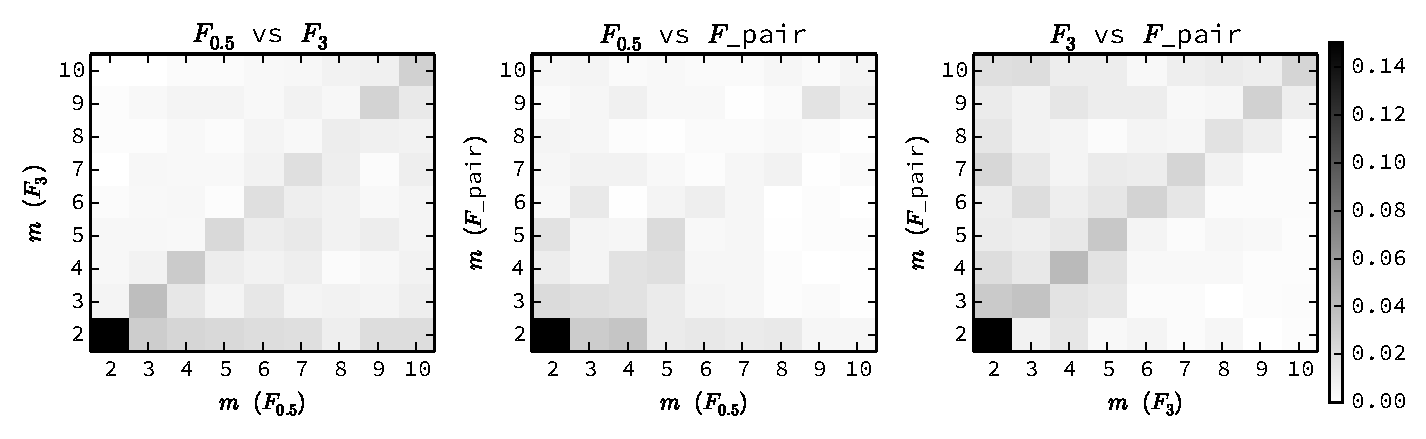
\includegraphics[width=0.9\textwidth]{figs/mconfusionfunc}
\caption{Confusion matrices illustrating the oracle selection of $m\in [2, 10]$ for 
different pairs of metrics on SALAMI (functional). While $m=2$ is most frequently
selected for all metrics, the large mass off-diagonal indicates that for a given
track, a single fixed $m$ does not generally optimize all evaluation metrics.\label{mconfusion}}
\end{figure*}

\section{Conclusions}
The experimental results in the previous section demonstrate that the proposed
structural decomposition technique often generates solutions which can achieve high
scores on segmentation evaluation metrics.  However, automatically selecting a single
``best'' segmentation without a priori knowledge of the evaluation criteria remains a
challenging practical issue.

\bibliography{refs}

\end{document}
